\chapter{Problembeschreibung und Optimalität}

\begin{definition}[Min-Cost-Flow-Problem (im Folgenden: MCFP)]
Ziel des \textbf{MCFP} ist es, eine Flussfunktion $f$ oder auch einen $b-Fluss$ in einem Flussnetzwerk zu finden, welche(-r) eine gegebene Kostenfunktion minimiert. Dabei soll die Zielfunktion die günstigste Möglichkeit für den Transport von einem oder mehreren Startpunkten (Quellen) durch ein Netzwerk zu einem oder mehreren Zielpunkten (Senken) repräsentieren. Kapazitätsbeschränkungen als auch Balancen im Graphen sollen dabei eingehalten werden.
\end{definition}
In diesem Kapitel soll darauf eingegangen werden, anhand welchen Kriteriums ein $b-Fluss$ in einem Flussnetz als minimal/optimal betrachtet werden kann. Dabei wird zu Erklärungszwecken auf komplexe Graphen verzichtet. Zunächst aber noch ein paar Erläuterungen, welche zum Verständnis des Optimalitätskriterium benötigt werden.

\section{Prinzip der Residualgraphen}
Das Prinzip des Residualgraphen oder auch Restgraphen ist bereits aus dem \textit{Maximaler-Fluss-Problem (MFP)} bekannt. Dabei handelt es sich um eine Art \textit{Zurücksende-Prinzip}. Es basiert auf der Überlegung, dass bereits versendete Einheiten auf dem gleichen Weg, auf dem sie gesendet wurden, auch wieder zurückgesendet werden könnten. In der Modellierung wird dann zu einem vorhandenen Fluss in einem gegebenen Flussnetz ein \textit{Residualgraph} oder auch \textit{Restgraph} erstellt, welcher die entsprechenden Rücksendewege als Rückwärtskanten beinhaltet. Wichtig ist, der Residualgraph repäsentiert den möglichen Fluss, welcher verändert werden kann, deshalb werden in diesem Graphen keine Flüsse eingezeichnet.
\begin{definition}[Residualgraph]
Der \textbf{Residualgraph $G^f$} eines Flussnetzes ist ein Graph, der zusätzliche mögliche Flüsse anzeigt. Wenn es einen Pfad von der Quelle zur Senke im Residualgraphen gibt, dann ist es möglich, einen Fluss hinzuzufügen bzw. vorhandenen Fluss zu erhöhen. Jede Kante eines Residualgraphen hat einen Wert, die \textbf{Residualkapazität}(Rest-Kapazität)  \textbf{$u^f$}, welche gleich der ursprünglichen Kapazität der Kante abzüglich des aktuellen Flusses ist.
\end{definition}
\begin{figure}[htb]
\centering
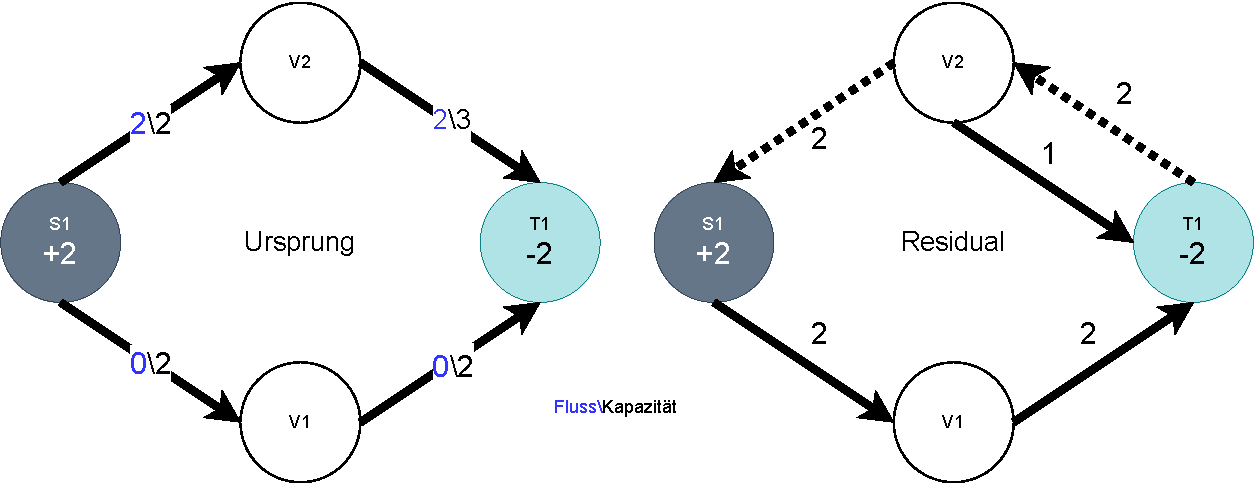
\includegraphics[width=0.9\textwidth]{img/steffen/simple_residual.drawio.pdf}
\caption{Einfacher Graph mit b-Fluss ($f1$) und korrespondierendem Residualgraph ($f1'$)}
\label{fig:simple_residual}
\end{figure}
In der Grafik \ref{fig:simple_residual} ist auf der linken Seite ein einfacher \textit{b-Fluss (S1, V2, T1)} in einem Graphen modelliert. Auf der rechten Seite ist der zugehörige Residualgraph abgebildet. Die Kanten, über die ursprünglich der \textit{b-Fluss} mit dem \textit{value=2} geflossen ist, werden nun als Rückwärtskanten dargestellt. Da auf der Kante \textit{E(V2,T1)} die Kapazität noch nicht voll ausgeschöpft ist, wird die Differenz aus Originalkapazität und vorhandenem Fluss auf der Vorwärtskante eingetragen.

\newpage
\subsection{Augmentierende Wege}
Innerhalb des Residualgraphen ist es unter Umständen möglich einen Weg von $s$ nach $t$ zu finden, über den ein Fluss > 0 gesendet werden kann, so dass der Gesamtfluss beeinflusst werden kann und weiterhin alle Kapazitätsgrenzen einhält. Ein solcher Weg wird als augmentierender Weg oder auch augmentierender Pfad bezeichnet.
\begin{definition}[Augmentierende Wege]
Ein Weg von $s$ nach $t$ im Residualgraph eines Flussnetzwerks heißt augmentierender Weg oder auch augmentierender Pfad wenn:
Der Weg von der Quelle zur Senke, entlang des Fluss weiter vergrößert(augmentiert) werden kann, ohne die Kapazitätsbeschränkungen der Kanten zu verletzen.
\end{definition}
\begin{figure}[htb]
\centering
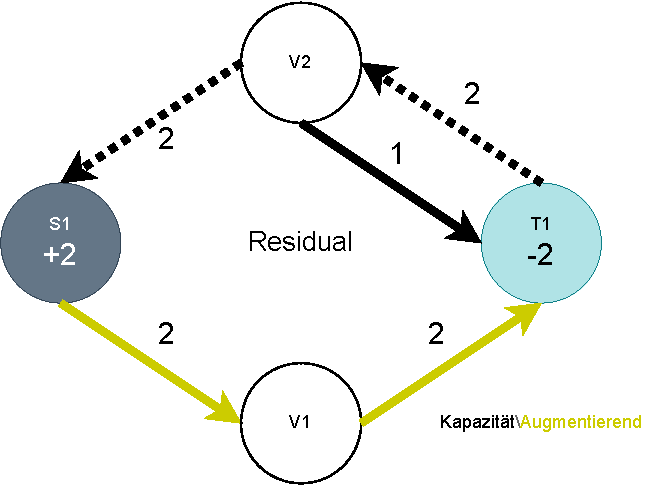
\includegraphics[width=0.7\textwidth]{img/steffen/augmented_way.drawio.pdf}
\caption{Augementierender Weg}
\label{fig:augmented_way}
\end{figure}
Die Grafik \ref{fig:augmented_way} zeigt in Gelb eingezeichnet einen augmentierenden Weg im Residualgraphen. Da im Ursprungsgraphen $G^f$ über diesen Weg noch keine Kapazitäten gesendet wurden, wäre es theoretisch möglich hier den Fluss zu erhöhen.

\subsection{Kosten}
Um das MCFP modellieren zu können, müssen Kosten abgebildet werden. Diese Kosten $c(e)$ in einem Graphen $G$ werden als Gewichtung an den Kanten dargestellt. Die Kosten können dabei exklusiv oder auch parallel zu anderen Gewichtungen existieren. Je nach Struktur der Kostenfunktion ist das zugrunde liegende Min-Cost-Flow-Problem \textit{np-hart} oder es existieren polynomiell exakte Algorithmen. Im Allgemeinen ist die Lösung von Min-Cost-Flow Problemen nicht eindeutig.
\begin{figure}[htb]
\centering
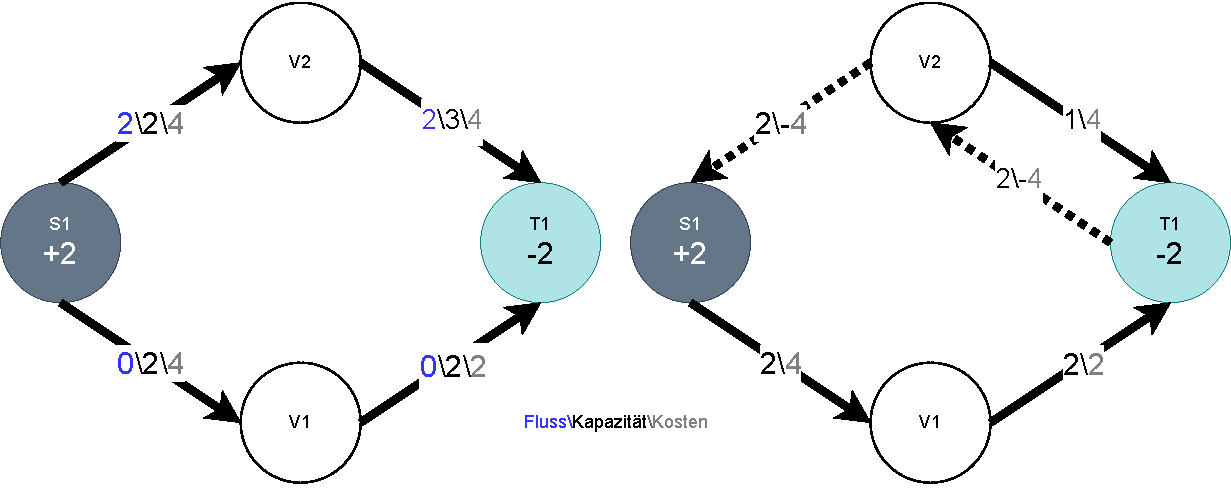
\includegraphics[width=1.0\textwidth]{img/steffen/graph_and_residual_with_costs.drawio.pdf}
\caption{Einfacher Graph mit b-Fluss($f1$), Kosten und zugehörigem Residualgraph ($f1'$)}
\label{fig:graph_and_residual_with_costs}
\end{figure}
Die Gesamtkosten von $f1$ in Abbildung \ref{fig:graph_and_residual_with_costs} entsprechen:
\begin{equation}
    f1 = 2*4 + 2*4 + 0*4 + 0*2 = 16
\end{equation}
%\textbf{Residualkosten}
\begin{definition}[Residualkosten $c^f$Satz 10.5]
Die Vorwärtskanten von Knoten im Residualgraphen bekommen die ursprünglichen Kosten zugewiesen und die Rückwärtskanten den negativen Wert ihrer Vorwärtskanten:
\begin{equation}
    \forall e \in E \quad c^f (e) = c(e) \Leftrightarrow c^f (\overleftarrow{e}) = -c(e)
\end{equation}
\end{definition}
Abbildung \ref{fig:graph_and_residual_with_costs} zeigt neben dem Originalgraphen auch den Residualgraphen mit bereits eingetragenen Kosten. Über die Kanten (S1, V2) und (V2, T1) fließt $b$ im Originalgraphen. Deshalb erhalten die Rückwärtskanten negative Kosten, die Vorwärtskanten behalten die originalen positiven Kosten.

\section{Lösung des MCFP mit Ford-Fulkerson?}

\textbf{Kann das MCFP durch den Ansatz von Ford-Fulkerson gelöst werden?} Sprich:
Kann durch sukzessives Erhöhen des Flusses mit Hilfe von (s-t)-Wegen aus dem Residualgraphen ein optimales Ergebnis für das MCFP gefunden werden? Welche Rolle spielt dabei die Kostenfunktion? Zunächst hier noch ein kurzer Rückblick auf die Optimalität von MFP:

\subsection{Optimalität von maximalen Flüssen}

Für das MFP war das Ziel in einem gegebenen Flussnetz (mit einer endlichen Menge an (s-t)-Flüssen) mindestens einen auszuwählen, für den die aus $s$ ausgehenden Flussmengen abzüglich der eingehenden Flussmengen maximal sind. Für diesen Fluss gilt das MFP als optimal. Formal ausgedrückt ist Kriterium für die Optimalität des MFP:
\begin{definition}[Satz 10.5]
    Ein (s, t)-Fluss $f$ oder auch b-Fluss ist genau dann maximal, wenn es \textbf{\textit{keinen f-augmentierenden Weg in $G^f$}} gibt. Dabei entspricht $G^f$ dem Residualgraphen.
\end{definition}
Mit anderen Worten: Erhöhe den Fluss in einem Graphen solange, bis aus dem Residualgraphen hervorgeht, dass keine weitere Flusserhöhung möglich ist.

\subsection{Augmentierende Wege und b-Flüsse}

Erwiesen ist, dass ein gegebener \textbf{(s-t)-Fluss} in einem Flussnetz systematisch verändert bzw. umgeleitet werden kann, ohne dabei Kapazitätsbeschränkungen zu verletzen. Das heißt auch, dass es möglich sein muss in einem Graphen für beliebige \textbf{(s-t)-Flüsse} einen auszuwählen, welcher ein zulässiger Fluss sein muss, aber auch möglichst niedrige Kosten haben kann. Aber gilt:
\begin{equation}
    \textbf{Maximaler-Fluss} = \textbf{b-Fluss} ???
\label{formular:st_flow_eq_b_flow}
\end{equation}

Schaubild \ref{fig:augmented_way} enthält einen f-augmentierenden Pfad durch den Residualgraphen $G^f$. Nach dem Vorgehen von Ford-Fulkerson würde der Fluss nun in einem resultierenden Graphen um 2 über den Weg (S1,V1,T1) erhöht werden.
\begin{figure}[htb]
\centering
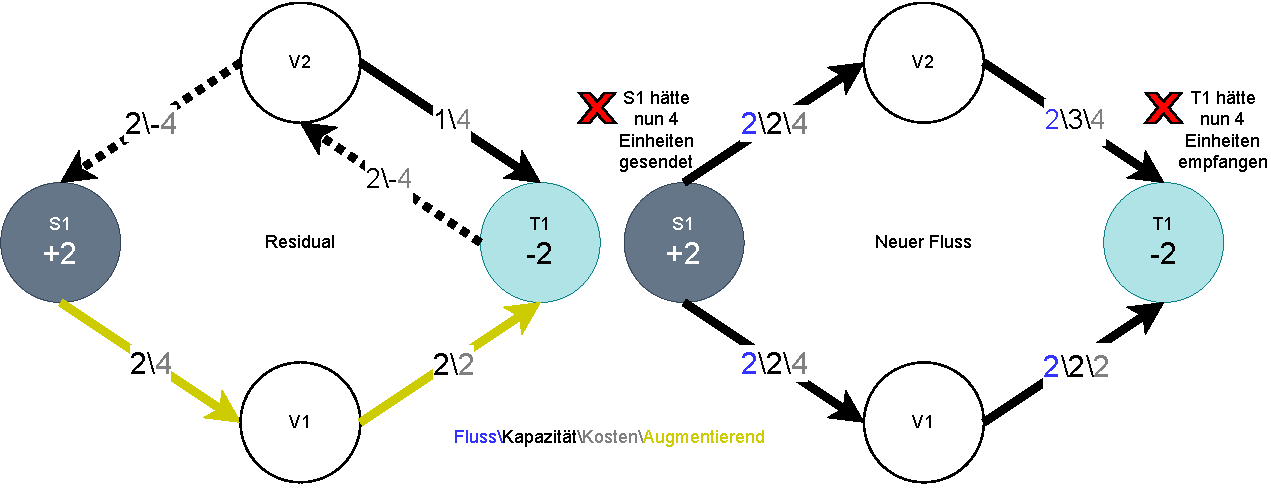
\includegraphics[width=1.0\textwidth]{img/steffen/augmented_way_with_resulting.drawio.pdf}
\caption{Residualgraph ($f1'$) mit augmentierendem Weg und resultierender Fluss ($f2$)}
\label{fig:augmented_way_with_resulting_graph}
\end{figure}
In der Veranschaulichung \ref{fig:augmented_way_with_resulting_graph} ist zu erkennen, dass direkt mehrere Probleme aus diesem Vorgehen entstehen:
\begin{itemize}
\item Weder die Balance von S1 noch T1 werden in $f2$ eingehalten
\item $c(f2)$ = \textbf{30 > 16} = $c(f1)$
\end{itemize}
Daraus lässt sich folgern, dass gilt:
\begin{equation}
    \textbf{Maximaler-Fluss} \neq \textbf{b-Fluss} !!!
\label{formular:st_flow_neq_b_flow}
\end{equation}
Weiterhin fällt es nicht schwer zu erkennen, dass die naive Anwendung von augmentierenden Pfaden nicht zu einer optimalen Lösung des MCFP führt.

\subsection{Kürzeste Wege und b-Flüsse}

Würde der ursprüngliche Fluss aus $f1$ über (S1, V2, T1) in Abbildung \ref{fig:invalid_b_flow} wegfallen, so wären die Balancen im Graphen wieder eingehalten und die resultierenden Kosten von $f2$ würden auf 12 sinken und damit wäre $c(f2)$ < $c(f1)$. Hinsichtlich der Forderung des MCFP nach minimalen Kosten wäre diese Option auf jeden Fall besser. Für den gegebenen Graphen ist dies sogar der optimale b-Fluss.
\begin{figure}[htb]
\centering
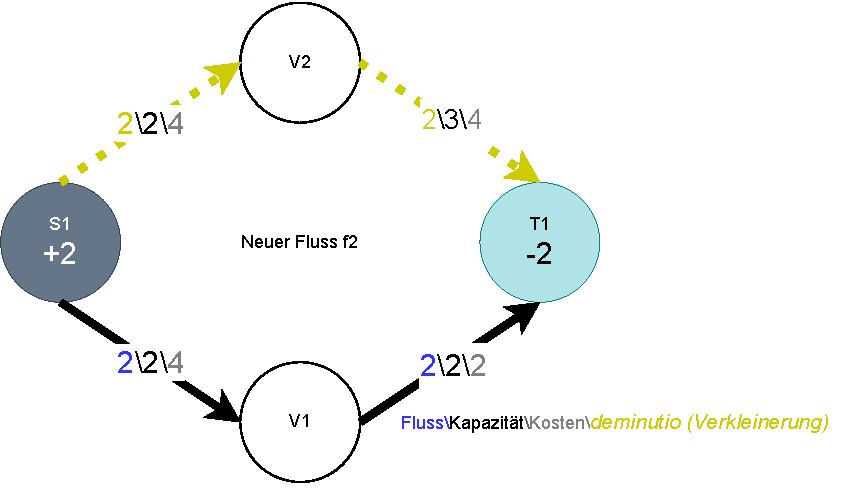
\includegraphics[width=0.6\textwidth]{img/steffen/invalid_b_flow.drawio.pdf}
\caption{(s-t)Fluss ($f2$) mit Weg, welcher die Balancen im Graphen verletzt.}
\label{fig:invalid_b_flow}
\end{figure}
Losgelöst kann der Minimale Kostenfluss in einem Graphen auch als kürzester Weg von $s$ nach $t$ bezüglich der Kosten betrachtet werden. Ein Pfad/Weg von $s$ nach $t$ ist genau dann ein kürzester Weg, wenn seine Gesamtkosten minimal sind. Gesucht ist also der Shortest Cost Flow $f$ in G, welcher im Graphen \ref{fig:invalid_b_flow} bereits in blau eingezeichnet ist. Es muss nur noch der gelbe Ursprungsfluss wieder zurück geleitet werden.
\begin{figure}[htb]
\centering
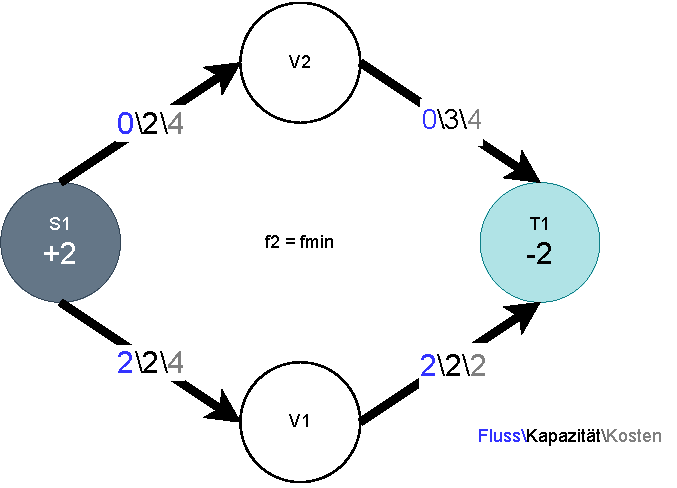
\includegraphics[width=0.6\textwidth]{img/steffen/min_cost_flow_graph.drawio.pdf}
\caption{$f2$ als Minimaler Kostenfluss in $G$}
\label{fig:min_cost_flow_graph}
\end{figure}
In dem Graphen \ref{fig:min_cost_flow_graph} ist der minimale Kostenfluss für das gegebene Flussnetz ohne den ursprünglichen Fluss eingetragen. Alle Bedingungen sind erfüllt. \textbf{Warum ist dies nun die optimale Lösung?}

\section{Augmentierende Zykel und Optimalität}

In der Gegenüberstellung der Residualgraphen von f1 und f2 (Abbildung \ref{fig:resi_f1_vs_f2}) sind jeweils zwei Zykel farblich hinterlegt.
\begin{definition}[Augmentierende Zykel]
Statt eines f-augmentierenden Wegs, der für maximale Flüsse benötigt wird, definieren wir nun einen f-augmentierenden Zykel Z. Ein f-augmentierender Zykel ist ein gerichteter Kreis in dem Residualgraphen $G^f$
\label{def:augmented_cycle}
\end{definition}
\begin{figure}[htb]
\centering
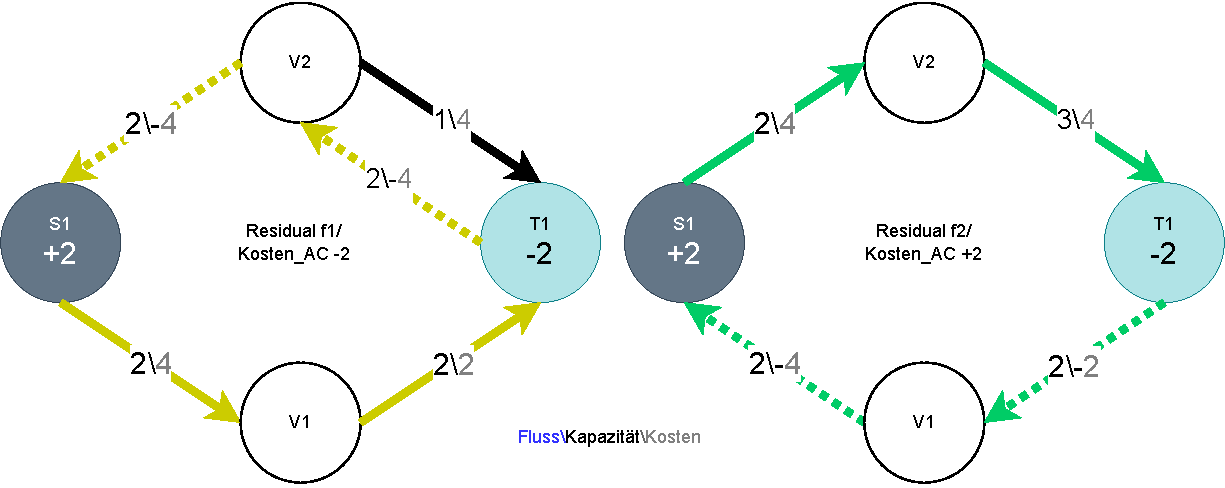
\includegraphics[width=1.0\textwidth]{img/steffen/resi_f1_vs_f2.drawio.pdf}
\caption{Residualgraph zu $f1$ gegenüber Residualgraph $f2$}
\label{fig:resi_f1_vs_f2}
\end{figure}
Summiert ergeben die Kosten entlang der farblich markierten Zykel jeweils \textit{c(f1') = -2} und \textit{c(f2') = 2}. Daraus lässt sich folgendes Vermuten (der formale Beweis der Optimalität wird hier aus Komplexitätsgründen bewusst ausgeklammert. Es darf davon ausgegangen werden, dass das Optimalitätskriterium gilt):

\begin{definition}[Satz 11.1 (Optimalitätskriterium für MCFP, Klein 1967).]
    Sei $G = (V, E)$ ein gerichteter Graph, $u$ die oberen Kantenkapazitäten, $c$ eine Kostenfunktion auf den Kanten und $b$ eine Balance. Dann ist $f$ genau dann ein kostenminimaler Fluss, wenn kein f-augmentierender Zykel $Z$ mit negativen Kosten in $G^f$ existiert.
\end{definition}

\subsection{Wie findet man negative Zykel?}

Um in einem Graphen einen minimalen Kostenfluss zu finden, ist es also essentiell Möglichkeiten bzw. Algorithmen zu haben, welche Zykel in Graphen erkennen können. Hier eine (nicht vollständige) Auflistung:

\begin{itemize}
\item \textbf{Moore-Bellman-Ford-Algorithmus O(n*m)}
\item Robust-Dijkstra-Algorithmus O(n*m)
\item Goldberg-Radzik-Algorithmus O(n*m)
\end{itemize}

Es fällt auf, dass es laut dieser Liste keinen Algorithmus gibt, welcher eine Komplexität von O(n*m) unterschreitet. Wurde ein negativer Zykel in einem Residualgraphen gefunden, kann dann durch Augmentieren eines b-Fluss $b1$ um den Wert $\gamma$  ein neuer b-Fluss $b2$ erzeugt werden, welcher den gefundenen Zykel nicht mehr beinhaltet.
\begin{equation}
    \gamma \leq min_{e\in Z} u^f(e)
\label{def:gamma}
\end{equation}
Es kann sein, dass der neue $b-Fluss$ weitere negative Zykel beinhaltet. Diese können dann iterativ aufgelöst werden. Bis kein weiterer Zykel mehr vorhanden ist (siehe auch: Cycle cancelling algorithm):

\[ f'(e) = \begin{cases}
 f(e) & \text{falls } e \notin Z \\
 f(e) + \gamma & \text{falls    } e \in Z\\
 f(e) - \gamma & \text{falls    } \overleftarrow{e} \in Z
\end{cases} \]
Bezogen auf Abbildung \ref{fig:resi_f1_vs_f2} bedeutet das, durch die Erhöhung des augmentierenden Zyklus in f1' um den Wert 2 entsteht f2. Der daraus resultierende Residualgraph f2' enthält nach der Augmentierung einen positiven Zykel.

\subsection{Welche Algorithmen lösen ein MCFP?}

Stand 2022-Mai sind diverse Algorithmen bekannt, welche das MCFP lösen können. Ein paar davon sind hier aufgelistet. 

\begin{itemize}
 \item \textbf{Cycle cancelling algorithm (negative cycle optimality)}
 \item \textbf{Successive Shortest Path algorithm (reduced cost optimality)}
 \item Out-of-Kilter algorithm (complimentary slackness)
 \item Push/Relabel algorithm
 \item Dual Cancel and Tighten
 \item Primal-Dual
\end{itemize}

Die ersten beiden werden in den folgenden Kapiteln näher betrachtet.


% \textbf{Exkurs}
% Die Anwendung des Lagrange-Multiplikator hat sich als nicht praktikabel erwiesen.
% \textit{Lineare Kostenfunktion}
% \begin{itemize}
%     \item Linear Programing
%     \item Simplex Algorithm
% \end{itemize}
% \textit{Konvexe Kostenfunktion}
% \begin{itemize}
%     \item Capacity-Scaling Algorithm --> Linearisierung
% \end{itemize}
% \textit{Allgemeine nichtlineare Kostenfunktion}
% \begin{itemize}
%     \item Für allgemeine nichtlineare Kostenfunktionen ist das Finden einer Lösung in einem Min-Cost-Flow-Problem NP-schwer.
% \end{itemize}